\documentclass[11pt,a4paper]{article}
\usepackage{fontspec}
\setmainfont{DejaVu Serif}
\usepackage{amsmath,amssymb,graphicx,booktabs,geometry,hyperref}
\geometry{margin=22mm}
\sloppy
\setlength{\emergencystretch}{3em}
\graphicspath{{results/}}
\begin{document}
\title{Експеримент 3: незалежні параметри та офсети}\author{}\date{27 жовтня 2026}\maketitle

\section*{Протокол}
База: повернутий квадрат, $h=0.25$, $r/h=2$, $n=2$,
поворот $20^\circ$, зсув $0.03$, вузли збігаються з центрами.
У кожній серії змінюється лише один фактор:
$h\in\{0.16,0.2,0.25,0.32\}$,
$\rho\in\{1,1.5,2,3\}$, $n\in\{1,2,3,4\}$,
зміщення вузлів $0,0.1h,0.25h$,
поворот $0,15,30,45^\circ$, зсув $0,0.04,0.10$,
офсет $t=-0.15,0,0.15$. Це окремі одновимірні серії,
тому взаємодії факторів ще не досліджено.
Для окремої серії $r=0.5$ при зміні $h$, отже $\rho$ змінюється.
Критичні офсети також досліджено на дисках, перешийку, колі та торі.
Рівень точної SDF --- $\{d=t\}$; рівень моделі --- $\{f=t\}$.
\[
 E_{\rm band}=\sqrt{\frac1{|B|}\sum_{x\in B}(f(x)-d(x))^2},
 \qquad B=\{x:|d(x)-t|<0.2\}.
\]
Ця метрика вимірює поле біля офсету. Вона не є безпосередньою
відстанню Гаусдорфа між офсетними поверхнями.
\begin{center}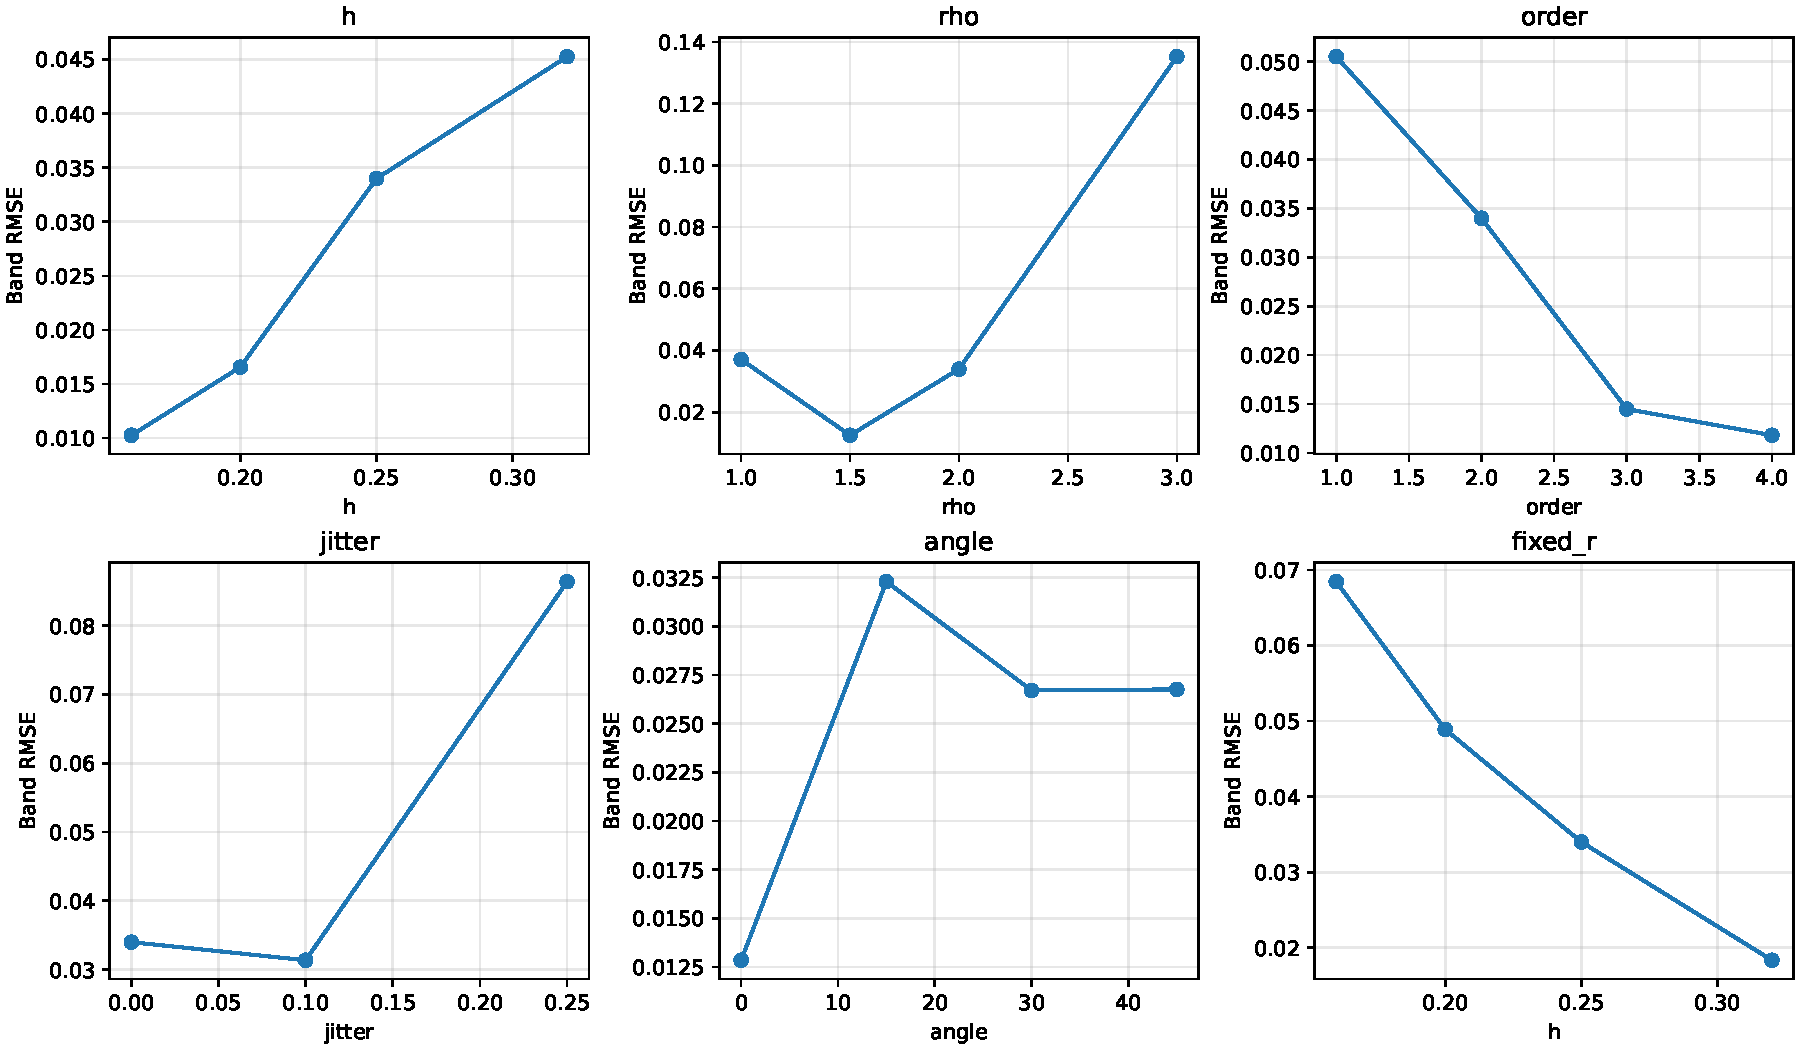
\includegraphics[width=\linewidth]{results/experiment3.pdf}\end{center}
Виконано 44 конфігурацій, успішних 44, відмов 0.
\begin{center}\small\resizebox{\linewidth}{!}{\begin{tabular}{llllll}\toprule
Форма & $t$ & RMSE смуги & Помилка знака & Компоненти d & Компоненти f\\\midrule
two\_circles & 0 & 0.0288 & 0.02342 & 2 & 2\\
two\_circles & 0.06 & 0.02833 & 0.02877 & 2 & 2\\
two\_circles & 0.08 & 0.02824 & 0.02781 & 2 & 1\\
two\_circles & 0.1 & 0.02824 & 0.02807 & 1 & 1\\
neck & -0.12 & 0.03269 & 0.01447 & 2 & 2\\
neck & -0.1 & 0.03249 & 0.02048 & 1 & 4\\
neck & -0.08 & 0.03219 & 0.03895 & 1 & 1\\
neck & 0 & 0.0327 & 0.05175 & 1 & 1\\
circle & -0.57 & 0.04778 & 0 & 0 & 0\\
circle & -0.55 & 0.04598 & 0 & 1 & 1\\
circle & -0.53 & 0.04317 & 0.002631 & 1 & 1\\
torus & -0.21 & 0.02987 & 0 & 0 & 0\\
torus & -0.19 & 0.02937 & 0.0003732 & 12 & 4\\
torus & 0.3 & 0.01768 & 0.01399 & 1 & 1\\
torus & 0.34 & 0.01793 & 0.01591 & 1 & 1\\
\bottomrule\end{tabular}}\end{center}
Диски зливаються при зовнішньому офсеті $t=0.08$;
перешийок руйнується поблизу внутрішнього офсету $t=-0.10$.
Коло зникає при $t<-0.55$; точно при $t=-0.55$ лишається точка.
Для тора $t=-0.20$ --- виродження трубки,
$t=R-a=0.32$ --- закриття центрального отвору.
Кількість зв'язних компонент не виявляє всіх змін роду тора.
При $t=-0.19$ радіус трубки лише $0.01$, тоді як крок оцінки
$2/34$. Тому навіть точний тор у цьому тесті розпадається на
сіткові компоненти. Це артефакт дискретизації, і його не можна
інтерпретувати як топологію неперервної SDF або як доведену
топологічну помилку інтерполянта.
При критичних значеннях дискретний тест особливо чутливий до сітки.
Геометрична зміна самого еталона не є помилкою інтерполяції.

За фіксованого $\rho$ кількість активних ядер обмежена
$O((1+\rho)^D)$; за сталого фізичного $r$ вона росте при
зменшенні $h$. Підвищення гладкості та зміна підтримки не утворюють
автоматично монотонного покращення. Час факторизації не входить
у вартість одного запиту. Дані \texttt{results/*.csv} містять
також час побудови, залишок у вузлах і число ненульових елементів.

\end{document}
